\subsection{GDI+}

Tak jak w Win32API istnieją funkcje GDI, tak w świecie .NET istnieje biblioteka GDI+, która
udostępnia obiektowy interfejs do funkcji GDI. 

Używając GDI+ programista musi pamiętać o jednej bardzo ważnej rzeczy. Otóż zainicjowanie obiektu
graficznego, takiego jak pędzel, szczotka, font, obiekt typu {\bf Graphics} itd., spowoduje
utworzenie odpowiedniego elementu w systemie, do którego uchwyt będzie przechowywany wewnątrz obiektu.

Interfejs GDI skonstruowany jest jednak tak, że gdy element graficzny przestaje być potrzebny, powinien
być usunięty, aby system mógł zwolnić zasoby związane z nim. W GDI+ rozwiązano ten problem tak, że
wszystkie obiekty graficzne implementują interfejs {\bf IDisposable}, zaś zasoby systemowe są
zwracane w metodzie {\bf Dispose}. Warto w tym miejscu przypomnieć sobie więc cukierek syntaktyczny
ze strony \pageref{disposeSyntaxSugar}, dzięki któremu programista nie musi pamiętać o wywołaniu
metody {\bf Dispose}.

\subsubsection{Obiekt {\bf Graphics}}

W GDI do narysowania czegokolwiek potrzebny był kontekst urządzenia. W GDI+ analogiczną rolę pełni
obiekt typu {\bf Graphics}. 

Obiekt ten jest dostarczany do wszystkich funkcji obsługujących
zdarzenia związane z rysowaniem w parametrze typu {\bf PaintEventArgs} i jest to pewna analogia
do obsługi zdarzenia WM\_PAINT w Win32API.

Obiekt ten może być również utworzony w dowolnej chwili działania aplikacji za pomocą statycznych funkcji
{\bf FromHdc}, {\bf FromHwnd} czy {\bf FromImage}.

Obiekt {\bf Graphics} potrafi wykonać większość operacji związanych z rysowaniem (wymagają wskazania
pędzla jako jednego z parametrów), m.in.:

\begin{itemize}
\item DrawArc
\item DrawBezier
\item DrawEllipse
\item DrawIcon
\item DrawImage
\item DrawLine
\item DrawPath
\item DrawPie
\item DrawRectangle
\item DrawString
\end{itemize}

oraz kilka funkcji związanych z wypełnianiem obszarów (wymagają szczotki jako parametru), m.in:

\begin{itemize}
\item FillEllipse
\item FillPie
\item FillRectangle
\item FillRegion
\end{itemize}

\subsubsection{Kolory}

W każdym miejscu, w którym potrzebne jest określenie koloru, należy skorzystać z obiektu {\bf Color}.
Klasa kolor ma predefiniowane około 140 nazw kolorów, dostępnych jako statyczne propercje, na przykład
{\bf Color.Black}, {\bf Color.AliceBlue}, czy {\bf Color.Red}. Oprócz tego istnieje klasa
{\bf SystemColors}, która udostępnia wartości kolorów przypisanych elementom interfejsu graficznego
Windows. Mamy tu więc m.in. {\bf SystemColors.ActiveBorder}, {\bf SystemColors.Control}, 
czy {\bf SystemColors.WindowText} (w sumie około 25 predefiniowanych kolorów).

W każdej chwili programista może utworzyć własny kolor, opisując jego składowe:

\begin{scriptsize}
\begin{verbatim}
Color c = Color.FromArgb( 40, 50, 60 );
\end{verbatim}
\end{scriptsize}

\subsubsection{Czcionki}

Konstruktor obiektu {\bf Font} pozwala na określenie parametrów czcionki m.in.: 
wielkości, stylu, zestawu znaków. Poniższy przykład jest interesujący również z innego powodu:
czcionka jest tworzona i usuwana, zaś obiekt {\bf Graphics} nie jest usuwany. Jak to wytłumaczyć?

Otóż zauważmy, że obiekt typu {\bf Graphics} jest dostarczony jako parametr w zmiennej typu 
{\bf PaintEventArgs}. Oznacza to, że jest on konstruowany gdzieś indziej. Również gdzieś indziej może
być więc wykorzystywany. Usunięcie go przez {\bf Dispose} mogłoby w szczególnym przypadku objawić się
trudnym do zdiagnozowania błędem.

W przeciwieństwie do obiektu {\bf Graphics}, czcionka jest konstruowana lokalnie i powinna być usunięta
po użyciu. 

\begin{scriptsize}
\begin{verbatim}
/* Wiktor Zychla, 2003 */
using System;
using System.Drawing;
using System.Windows.Forms;

namespace Example
{
  public class CMainForm : Form
  {  
    public CMainForm() {}

    protected override void OnPaint( PaintEventArgs e )
    {
      Graphics g = e.Graphics;

      using ( Font f = new Font( "Courier", 24, FontStyle.Italic ) )
      {
        g.DrawString( "Przykład GDI+", f, Brushes.Black, 0, 0 );
      }
    }

    public static void Main()
    {    
      Application.Run( new CMainForm() );
    }
  }
}
\end{verbatim}
\end{scriptsize}

\subsubsection{Pędzle, szczotki}

GDI+ dostarcza całego zestawu gotowych pędzli i szczotek w obiektach {\bf Pens} i {\bf Brushes}.
W każdym miejscu kodu można z nich skorzystać, a jest to o tyle łatwe, że nazwano je po prostu
nazwami kolorów. Mamy więc na przykład pióro czarne {\bf Pens.Black} czy szczotkę niebieską
{\bf Brushes.Blue}.

Oprócz gotowych piór i szczotek, programista może tworzyć własne. Konstruktor pióra przyjmuje jako parametr
kolor i opcjonalnie grubość pióra:

\begin{scriptsize}
\begin{verbatim}
/* Wiktor Zychla, 2003 */
using System;
using System.Drawing;
using System.Windows.Forms;

namespace Example
{
  public class CMainForm : Form
  {  
    public CMainForm() {}

    protected override void OnPaint( PaintEventArgs e )
    {
      Graphics g = e.Graphics;

      using ( Pen p = new Pen( Color.FromArgb( 40, 50, 130 ), 5 ) )
      {
        g.DrawLine( p, 0, 0, 50, 50 );
      }
    }

    public static void Main()
    {    
      Application.Run( new CMainForm() );
    }
  }
}
\end{verbatim}
\end{scriptsize}

W przypadku szczotek możliwości jest trochę więcej. Istnieje klasa bazowa {\bf Brush}, z której
wyprowadzono klasy umożliwiające tworzenie róznego rodzaju szczotek: {\bf SolidBrush},
{\bf HatchBrush}, {\bf LinearGradientBrush}, {\bf PathGradientBrush} czy {\bf TextureBrush}.

Zobaczmy na przykład jak za pomocą szczotki gradientowej wyposażyć okno w automatycznie odrysowywane
gradientowe tło:

\begin{figure}
\begin{center}
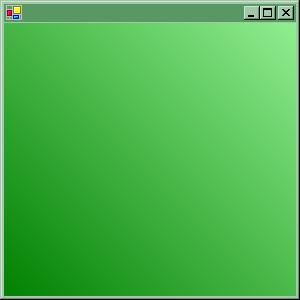
\includegraphics[width=0.50\textwidth]{./pic/swf05}
\caption{Gradientowe tło uzyskane dzięki odpowiedniej szczotce}
\end{center}
\end{figure}

\begin{scriptsize}
\begin{verbatim}
/* Wiktor Zychla, 2003 */
using System;
using System.Drawing;
using System.Drawing.Drawing2D;
using System.Windows.Forms;

namespace Example
{
  public class CMainForm : Form
  {  
    public CMainForm() {}

    protected override void OnPaint( PaintEventArgs e )
    {
      Graphics g = e.Graphics;

      using ( LinearGradientBrush lgb = 
        new LinearGradientBrush( this.ClientRectangle, Color.Green, 
                                 Color.LightGreen, -45f, false ) )
      {
        g.FillRectangle( lgb, this.ClientRectangle );
      }
    }

    protected override void OnResize( EventArgs e )
    {
      Invalidate();
    } 

    public static void Main()
    {    
      Application.Run( new CMainForm() );
    }
  }
}
\end{verbatim}
\end{scriptsize}

\subsubsection{Obrazki}

Tworzenie obrazków możliwe jest dzięki dwóm klasom: {\bf Image} i dziedziczącej z niej {\bf Bitmap}.
Obrazek może być utworzony dynamiczne bądź załadowany z pliku ({\bf Image.FromFile}). 
Obrazek w pamięci można poddać różnym operacjom, można nawet utworzyć obiekt {\bf Graphics} dzięki funkcji
{\bf Graphics.FromImage} i rysować na powierzchni obrazka za pomocą funkcji z GDI+.

Gotowy obrazek można zapisać za pomocą metody {\bf Save}, wybierając przy okazji jeden z dostępnych formatów m.in.
GIF, BMP, PNG, JPG.

Zawartość obrazka można dzięki funkcji {\bf DrawImage} obiektu {\bf Graphics} narysować w kontekście, na który
wskazuje obiekt {\bf Graphics} lub umieścić w komponencie typu {\bf PictureBox}, który może być umieszczony
w oknie. Komponent {\bf PictureBox} sam dba o automatycznie odświeżanie swojej zawartości, programista nie musi
więc odrysowywać zawartości obrazka gdy okno wymaga odświeżenia.

\subsubsection{Podwójne buforowanie}

GDI+ udostępnia możliwość automatycznego podwójnego buforowania wyświetlanej grafiki. Dzięki
temu obraz rysowany jest na niewidocznej stronie graficznej i jest błyskawicznie przenoszony na
powierzchnię okna. Podwójne buforowanie umożliwia całkowite wyeliminowanie efektu "migania" obrazu
podczas rysowania. 

Aktywowanie podwójnego bufowania wymaga jedynie 3 lini kodu w konstruktorze okna:

\begin{scriptsize}
\begin{verbatim}
/* Wiktor Zychla, 2003 */
this.SetStyle(ControlStyles.UserPaint, true);
this.SetStyle(ControlStyles.AllPaintingInWmPaint, true);
this.SetStyle(ControlStyles.DoubleBuffer, true);
\end{verbatim}
\end{scriptsize}

\subsection{Zegary}

Oprogramowanie zegarów jest bardzo proste, ponieważ wystarczy utworzyć obiekt typu {\bf Timer}, 
przypiąć funkcję do listy słuchaczy zdarzenia {\bf Tick} i ustalić interwał czasu między kolejnymi 
zgłoszeniami zdarzenia.

\begin{figure}
\begin{center}
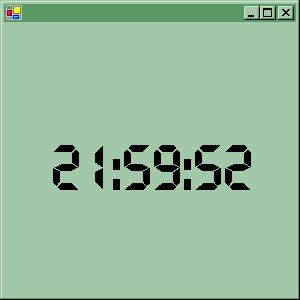
\includegraphics[width=0.50\textwidth]{./pic/swf01}
\caption{Zegarek w C\# z podwójnym buforowaniem grafiki}
\end{center}
\end{figure}

\label{kodZegarek}

\begin{scriptsize}
\begin{verbatim}
/* Wiktor Zychla, 2003 */
using System;
using System.Drawing;
using System.Windows.Forms;

namespace Example
{
  public class CMainForm : Form
  {   
    Timer timer;    

    public CMainForm()
    {
      timer          = new Timer();
      timer.Tick    += new EventHandler( Timer_Tick );
      timer.Interval = 50;
      timer.Start();

      this.SetStyle(ControlStyles.UserPaint, true);
      this.SetStyle(ControlStyles.AllPaintingInWmPaint, true);
      this.SetStyle(ControlStyles.DoubleBuffer, true);
    } 

    void Timer_Tick( object sender, EventArgs e )
    {              
      this.Invalidate();
    }

    protected override void OnPaint( PaintEventArgs e )
    {
      Graphics g = e.Graphics;
      using ( Font f = new Font( "LED", 48 ) )
      {
        StringFormat sf  = new StringFormat();
        sf.Alignment     = StringAlignment.Center;
        sf.LineAlignment = StringAlignment.Center;

        g.Clear( SystemColors.Control );
        g.DrawString( DateTime.Now.ToLongTimeString(), f, Brushes.Black, 
                      this.Width / 2, this.Height / 2, sf );
      }
    }

    public static void Main()
    {
      Application.Run( new CMainForm() );
    }
  }
}
\end{verbatim}
\end{scriptsize}

